\documentclass[11pt]{article}

% ============================================================
% Milestone 2 -- Progress Report (template 6.2)
% DIP Team Project (CSE681), project C21
%
% Every number in the text is a macro from generated/numbers.tex, and every
% results table is generated. To update after new runs:
%   uv run python scripts/export_report_assets.py
% Build: pdflatex main && bibtex main && pdflatex main && pdflatex main
% ============================================================
\usepackage[margin=1in]{geometry}
\usepackage[T1]{fontenc}
\usepackage[utf8]{inputenc}
\usepackage{amsmath,amssymb}
\usepackage{graphicx}
\usepackage{booktabs}
\usepackage[round]{natbib}
\usepackage{hyperref}
\hypersetup{colorlinks=true, linkcolor=blue!50!black, citecolor=blue!50!black, urlcolor=blue!50!black}
\usepackage{xurl}
\usepackage{enumitem}
\usepackage{xcolor}
\usepackage{caption}
\usepackage{array}

\newcommand{\todo}[1]{\textcolor{red}{\textbf{[TODO: #1]}}}
% Generated by scripts/export_report_assets.py. Do not edit by hand: rerun the script.
% Noise level: medium; seed 42.
\newcommand{\NoisyPSNR}{19.77}
\newcommand{\NoisyPSNRsd}{0.68}
\newcommand{\NoisySSIM}{0.249}
\newcommand{\NoisyDp}{0.295}
\newcommand{\NoisyAgr}{0.574}
\newcommand{\NoisyLost}{81.7\%}
\newcommand{\NoisyNew}{29.5\%}
\newcommand{\NoisyDAUC}{$+0.158$}
\newcommand{\NoisyDAUCci}{[$+0.096$, $+0.225$]}
\newcommand{\MedianPSNR}{26.77}
\newcommand{\MedianPSNRsd}{0.67}
\newcommand{\MedianSSIM}{0.553}
\newcommand{\MedianDp}{0.353}
\newcommand{\MedianAgr}{0.372}
\newcommand{\MedianLost}{6.3\%}
\newcommand{\MedianNew}{81.6\%}
\newcommand{\MedianDAUC}{$+0.143$}
\newcommand{\MedianDAUCci}{[$+0.090$, $+0.196$]}
\newcommand{\MedianGain}{7.0}
\newcommand{\BMPSNR}{33.51}
\newcommand{\BMPSNRsd}{0.99}
\newcommand{\BMSSIM}{0.884}
\newcommand{\BMDp}{0.096}
\newcommand{\BMAgr}{0.805}
\newcommand{\BMLost}{10.7\%}
\newcommand{\BMNew}{22.4\%}
\newcommand{\BMDAUC}{$+0.051$}
\newcommand{\BMDAUCci}{[$+0.017$, $+0.080$]}
\newcommand{\BMGain}{13.7}
\newcommand{\OursPSNR}{34.47}
\newcommand{\OursPSNRsd}{1.09}
\newcommand{\OursSSIM}{0.912}
\newcommand{\OursDp}{0.056}
\newcommand{\OursAgr}{0.898}
\newcommand{\OursLost}{28.5\%}
\newcommand{\OursNew}{4.1\%}
\newcommand{\OursDAUC}{$+0.017$}
\newcommand{\OursDAUCci}{[$-0.005$, $+0.036$]}
\newcommand{\OursGain}{14.7}
\newcommand{\BMSec}{2.6}
\newcommand{\BMMinutes}{26}
\newcommand{\BMHardware}{CPU, 4 workers}
\newcommand{\OursMs}{1.5}
\newcommand{\GPUName}{NVIDIA RTX PRO 2000 Blackwell Generation Laptop GPU}
\newcommand{\Speedup}{1{,}732}
\newcommand{\CmpPSNR}{$+0.96$}
\newcommand{\CmpPSNRci}{[$+0.94$, $+0.99$]}
\newcommand{\CmpPSNRShare}{100\%}
\newcommand{\CmpSSIM}{$+0.027$}
\newcommand{\CmpSSIMci}{[$+0.027$, $+0.028$]}
\newcommand{\CmpSSIMShare}{100\%}
\newcommand{\CmpDp}{$-0.041$}
\newcommand{\CmpDpci}{[$-0.045$, $-0.036$]}
\newcommand{\CmpDpShare}{77\%}
\newcommand{\CmpAgr}{$+0.093$}
\newcommand{\CmpAgrci}{[$+0.080$, $+0.106$]}
\newcommand{\CmpAgrShare}{62\%}
\newcommand{\CmpAUC}{$+0.034$}
\newcommand{\CmpAUCci}{[$+0.009$, $+0.057$]}
\newcommand{\OursAUC}{0.724}
\newcommand{\BMAUC}{0.690}
\newcommand{\CmpDpRel}{42\%}
\newcommand{\MinPos}{20}
\newcommand{\NumAUCDiseases}{5}
\newcommand{\AUCDiseases}{Atelectasis, Effusion, Infiltration, Nodule and Pleural Thickening}
\newcommand{\OursNoduleDAUC}{$-0.020$}
\newcommand{\OursNoduleDAUCci}{[$-0.086$, $+0.038$]}
\newcommand{\BMLostNodule}{4\%}
\newcommand{\BMNewNodule}{52\%}
\newcommand{\OursLostNodule}{52\%}
\newcommand{\OursNewNodule}{2\%}
\newcommand{\BMLostMass}{0\%}
\newcommand{\BMNewMass}{76\%}
\newcommand{\OursLostMass}{8\%}
\newcommand{\OursNewMass}{25\%}
\newcommand{\BMLostFibrosis}{2\%}
\newcommand{\BMNewFibrosis}{69\%}
\newcommand{\OursLostFibrosis}{19\%}
\newcommand{\OursNewFibrosis}{11\%}
\newcommand{\BMShiftAll}{$+0.070$}
\newcommand{\BMShiftFindings}{$-0.014$}
\newcommand{\BMShiftNonFindings}{$+0.098$}
\newcommand{\OursShiftAll}{$-0.019$}
\newcommand{\OursShiftFindings}{$-0.056$}
\newcommand{\OursShiftNonFindings}{$-0.007$}
\newcommand{\JudgeFindings}{2{,}103}
\newcommand{\JudgePairs}{8{,}400}
\newcommand{\JudgeFindingsPct}{25.0\%}
\newcommand{\JudgeLowDp}{0.294}
\newcommand{\JudgeLowLost}{74\%}
\newcommand{\JudgeLowDAUC}{$+0.114$}
\newcommand{\JudgeMediumDp}{0.295}
\newcommand{\JudgeMediumLost}{82\%}
\newcommand{\JudgeMediumDAUC}{$+0.158$}
\newcommand{\JudgeHighDp}{0.280}
\newcommand{\JudgeHighLost}{86\%}
\newcommand{\JudgeHighDAUC}{$+0.194$}
\newcommand{\JudgeMedianAUC}{0.798}
\newcommand{\NoiseLowPSNR}{22.67}
\newcommand{\NoiseMediumPSNR}{19.77}
\newcommand{\NoiseHighPSNR}{16.91}
\newcommand{\TrainEpochs}{30}
\newcommand{\BestEpoch}{30}
\newcommand{\ValPSNR}{34.51}
\newcommand{\TrainMinutes}{4.7}
\newcommand{\SecPerEpoch}{9.5}
\newcommand{\Params}{449{,}489}
\newcommand{\NTrain}{2{,}000}
\newcommand{\PatTrain}{1{,}330}
\newcommand{\NoFindTrain}{69.1\%}
\newcommand{\NVal}{400}
\newcommand{\PatVal}{264}
\newcommand{\NoFindVal}{71.2\%}
\newcommand{\NTest}{600}
\newcommand{\PatTest}{405}
\newcommand{\NoFindTest}{68.3\%}
\newcommand{\NPatients}{1{,}999}
\newcommand{\Seed}{42}
\newcommand{\MaxPerPatient}{2}
\newcommand{\NAvailable}{24{,}999}
\newcommand{\NoFindFull}{53.8\%}
\newcommand{\NFull}{112{,}120}
\newcommand{\PatFull}{30{,}805}


\title{\LARGE Progress Report \\[4pt]
\large Diagnostic-Preserving Denoising for Low-Dose Medical Images}
\author{
  Omar Hesham Hanafy Mohamed Nasr (2401812) \and
  Mohamed Ahmed Abdelsalaam (2400033)
}
\date{Milestone 2 --- November 2026 \\{} CSE681 --- Digital Image Processing \\[6pt]
\normalsize \textbf{Code Repository:} \url{https://github.com/omarhesham1997/Diagnostic-Preserving-Denoising-for-Low-Dose-Medical-Images}}

\begin{document}
\maketitle

\begin{abstract}
We study whether denoising low-dose chest radiographs preserves the information a diagnostic classifier relies on. On a patient-disjoint subset of NIH ChestX-ray14 (\NTrain/\NVal/\NTest{} images) corrupted with simulated Poisson-Gaussian noise, we reproduced a median filter and Anscombe-BM3D, trained a \Params-parameter residual U-Net, and scored every method with pixel metrics and with a frozen TorchXRayVision DenseNet-121. At the medium noise level (\NoiseMediumPSNR\,dB input PSNR), the ResU-Net improves on BM3D by \CmpPSNR\,dB and lowers the classifier's mean probability change from \BMDp{} to \OursDp; its macro $\Delta$AUC of \OursDAUC{} \OursDAUCci{} has a confidence interval that includes zero. However, it removes \OursLost{} of the findings the classifier reports on clean images (\OursLostNodule{} of nodule findings), compared with \BMLost{} for BM3D: averaged metrics hide a systematic loss of small findings, which defines the main target for Milestone~3.
\end{abstract}

% ------------------------------------------------------------
\section{Recap}
\label{sec:recap}
Low-dose radiography reduces patient exposure but adds signal-dependent quantum noise and detector noise. Denoisers are usually judged by PSNR and SSIM \citep{wang2004ssim}, which weight every pixel equally and can reward smoothing that erases subtle findings. Following the task-aware evaluation idea of \citet{dai2025compression}, we evaluate denoisers on two families of metrics: pixel fidelity, and \emph{diagnostic preservation}, i.e.\ how much the predictions of a frozen chest X-ray classifier \citep{cohen2022torchxrayvision} change between the clean and the denoised image. We use NIH ChestX-ray14 \citep{wang2017chestxray8} with synthetic Poisson-Gaussian noise (paired real low/high-dose radiographs are not publicly available), Anscombe-BM3D \citep{dabov2007bm3d,makitalo2013gat} and a $3\times3$ median filter as classical baselines, and a lightweight residual U-Net \citep{ronneberger2015unet,zhang2017dncnn} as our method. The scope is unchanged from Milestone~1; the measurement protocol was extended (Section~\ref{sec:challenges}).

% ------------------------------------------------------------
\section{Implementation Status}
\label{sec:status}
The full pipeline runs end to end from the repository: data selection, preprocessing, noise simulation, the two baselines, the frozen classifier, training, evaluation, statistical comparison, figures, and the tables in this report (Table~\ref{tab:components}). Every step is a script with a fixed seed (\Seed); fixed noisy validation and test sets are stored once and reused by every method. The repository has an automated test suite (over 100 tests) (noise statistics, variance stabilization, split integrity, metric correctness, model shape and checkpoints), a locked environment (\texttt{uv.lock}, exported to \texttt{requirements.txt}), and a committed split file (\texttt{splits/split\_seed42.csv}).

\begin{table}[htbp]
\centering
\small
\caption{Implemented components. ``Verified by'' lists the automated check or experiment that confirms each component works.}
\label{tab:components}
\begin{tabular}{@{}p{0.22\linewidth}p{0.42\linewidth}p{0.29\linewidth}@{}}
\toprule
\textbf{Component} & \textbf{Implementation} & \textbf{Verified by} \\
\midrule
Data subset \& split & Patient-level split, at most \MaxPerPatient{} images per patient, seed \Seed & Tests: no patient in two splits, exact sizes, reproducible file \\
Noise simulation & Poisson-Gaussian model, one seed per image, unclipped & Tests: mean and variance match the model \\
Anscombe-BM3D & Generalized Anscombe transform in photon counts, BM3D, closed-form unbiased inverse & Tests: stabilized std within 0.95--1.05; inverse bias $<0.0015$ \\
Median filter & $3\times3$ median & Test: removes impulses \\
Frozen classifier & TorchXRayVision \texttt{densenet121-res224-all} & Clean-image AUCs (Table~\ref{tab:judgeauc}) \\
ResU-Net & M1 design, \Params{} parameters & Overfit test, training curves (Fig.~\ref{fig:training}) \\
Evaluation & PSNR, SSIM, $\Delta p$, agreement, lost/new findings, $\Delta$AUC with bootstrap CIs, paired tests & Tests on synthetic predictions \\
\bottomrule
\end{tabular}
\end{table}

\subsection{Data and Simulated Noise}
\label{sec:data}
\paragraph{Subset.} We used the labelled images of the first three NIH archive folders (\NAvailable{} images). Patients were visited in a seeded random order and contributed at most \MaxPerPatient{} randomly chosen images each, until \NTrain/\NVal/\NTest{} images were assigned to train/validation/test with no patient in two splits (\NPatients{} patients in total, Table~\ref{tab:dataset}). Images were converted to grayscale, resized from $1024\times1024$ to $256\times256$ (Lanczos), and scaled to $[0,1]$. Capping images per patient down-weights patients with many follow-up scans, who tend to be sicker: the subset contains more ``No Finding'' images (\NoFindTest{} in the test split) than the full dataset (\NoFindFull). Only \NumAUCDiseases{} diseases have at least \MinPos{} positive test cases (\AUCDiseases), so label-based metrics are restricted to them.

\begin{table}[htbp]
\centering
\caption{Dataset split (images, unique patients, share without any finding, and positive cases for the diseases used in $\Delta$AUC).}
\label{tab:dataset}
\resizebox{\linewidth}{!}{\begin{tabular}{@{}lrrrrrrrr@{}}
\toprule
\textbf{Split} & \textbf{Images} & \textbf{Patients} & \textbf{No Finding} & \textbf{Atelectasis} & \textbf{Effusion} & \textbf{Infiltration} & \textbf{Nodule} & \textbf{Pleural Thickening} \\
\midrule
Train & 2{,}000 & 1{,}330 & 69.1\% & 136 & 100 & 198 & 76 & 46 \\
Val & 400 & 264 & 71.2\% & 19 & 22 & 28 & 22 & 7 \\
Test & 600 & 405 & 68.3\% & 47 & 38 & 50 & 21 & 20 \\
\midrule
\textit{Total} & 3{,}000 & 1{,}999 & 69.2\% & 202 & 160 & 276 & 119 & 73 \\
\bottomrule
\end{tabular}
}
\end{table}

\paragraph{Noise.} A clean image $x\in[0,1]$ is corrupted as
\begin{equation}
  y = \frac{\mathcal{P}(\lambda x)}{\lambda} + \mathcal{N}(0,\sigma^2),
  \label{eq:noise}
\end{equation}
so the noise variance $x/\lambda + \sigma^2$ grows with brightness. The noisy image is \emph{not} clipped, because clipping distorts exactly the statistics the Anscombe transform relies on; only method outputs are clipped to $[0,1]$. Image $i$ of a split always receives seed $s_0 + i$, so all methods are evaluated on identical noisy images. Table~\ref{tab:noise} gives the measured quality of the noisy test images for the three levels planned in Milestone~1.

\begin{table}[htbp]
\centering
\caption{Measured quality of the noisy test images (\NTest{} images, mean $\pm$ standard deviation). These replace the estimates of Milestone~1 (Section~\ref{sec:challenges}).}
\label{tab:noise}
\begin{tabular}{@{}lcccc@{}}
\toprule
\textbf{Level} & $\boldsymbol{\lambda}$ & $\boldsymbol{\sigma}$ & \textbf{PSNR (dB)} & \textbf{SSIM} \\
\midrule
Low & 100 & 0.01 & 22.67 $\pm$ 0.74 & 0.363 $\pm$ 0.083 \\
Medium & 50 & 0.02 & 19.77 $\pm$ 0.68 & 0.249 $\pm$ 0.069 \\
High & 25 & 0.04 & 16.91 $\pm$ 0.60 & 0.157 $\pm$ 0.047 \\
\bottomrule
\end{tabular}

\end{table}

\subsection{Baseline Reproduction}
\label{sec:baselines}
\paragraph{Anscombe-BM3D.} Following \citet{makitalo2013gat}, the noisy image is converted to photon counts $z=\lambda y$ (read-noise standard deviation $\lambda\sigma$) and stabilized with the generalized Anscombe transform
\begin{equation}
  f(z) = 2\sqrt{\max\!\left(z + \tfrac{3}{8} + (\lambda\sigma)^2,\ 0\right)},
\end{equation}
after which the noise has standard deviation close to 1 at every brightness. The stabilized image is rescaled to $[0,1]$, denoised with BM3D \citep{dabov2007bm3d} (Python \texttt{bm3d} package, noise standard deviation rescaled accordingly), and mapped back with the closed-form approximation of the exact unbiased inverse. BM3D is given the true noise parameters, as our network is trained at the known noise level. Automated tests confirm that the stabilized noise has a standard deviation between 0.95 and 1.05 for brightness 0.02 to 1.0 at all three levels, and that the inverse is unbiased to within 0.0015.

\paragraph{Median filter.} A $3\times3$ median filter is applied to the noisy image.

\paragraph{Baseline results.} At the medium level, BM3D raises PSNR from \NoisyPSNR\,dB to \BMPSNR\,dB (+\BMGain\,dB) and the median filter to \MedianPSNR\,dB (+\MedianGain\,dB) (Table~\ref{tab:main}). The large margin of the non-local method over the local filter on smooth radiographs is the expected ordering. BM3D is the slowest component: \BMSec\,s per image (\BMHardware), about \BMMinutes\,minutes for the test set.

\subsection{Frozen Classifier and Diagnostic Metrics}
\label{sec:judge}
The classifier $g$ is TorchXRayVision's DenseNet-121 \citep{huang2017densenet,cohen2022torchxrayvision} with \texttt{densenet121-res224-all} weights, kept frozen. Its outputs are calibrated so that 0.5 is the model's own operating point for each disease; we use the 14 NIH outputs. Inputs are clipped to $[0,1]$, resized to $224\times224$ (antialiased bilinear) and scaled to $[-1024,1024]$ as the library expects. On clean test images its median AUC over diseases is \JudgeMedianAUC{} (Table~\ref{tab:judgeauc}). These AUCs are optimistic, because the weights were trained partly on NIH data; all our diagnostic metrics compare the classifier with itself (clean vs.\ processed) or report differences, which this affects much less.

For a clean image $x$ and an output $\hat{x}$ we report, as planned: the mean absolute probability change $\Delta p=\frac{1}{14}\sum_k |g_k(\hat{x})-g_k(x)|$ and the agreement of yes/no decisions at 0.5. We added two pooled rates that show the \emph{direction} of changes (Section~\ref{sec:challenges}):
\begin{equation}
  \text{Lost} = \frac{\#\{(i,k): g_k(x_i)\ge 0.5,\ g_k(\hat{x}_i)<0.5\}}{\#\{(i,k): g_k(x_i)\ge 0.5\}}, \qquad
  \text{New} = \frac{\#\{(i,k): g_k(x_i)< 0.5,\ g_k(\hat{x}_i)\ge0.5\}}{\#\{(i,k): g_k(x_i)<0.5\}},
\end{equation}
i.e.\ the share of the classifier's clean-image findings that disappear, and the share of its clean-image non-findings that become findings. On clean images the classifier reports \JudgeFindings{} findings over \JudgePairs{} image-disease pairs (\JudgeFindingsPct). Finally, $\Delta\mathrm{AUC}_k=\mathrm{AUC}_k(x)-\mathrm{AUC}_k(\hat{x})$ against the dataset labels, for the \NumAUCDiseases{} diseases with at least \MinPos{} test cases, with 95\% confidence intervals from a paired bootstrap over images (1{,}000 resamples, \citealp{efron1993bootstrap}); ``macro'' is the average over these diseases. Two methods are compared on the same images with a paired bootstrap of the mean difference and a Wilcoxon signed-rank test \citep{wilcoxon1945}.

\begin{table}[htbp]
\centering
\small
\caption{Frozen classifier on the clean test images. Diseases with fewer than \MinPos{} cases have unstable AUCs and are not used for $\Delta$AUC.}
\label{tab:judgeauc}
\begin{tabular}{@{}lrcc@{}}
\toprule
\textbf{Disease} & \textbf{Test cases} & \textbf{AUC (clean)} & \textbf{Used for $\Delta$AUC} \\
\midrule
Infiltration & 50 & 0.654 & yes \\
Atelectasis & 47 & 0.748 & yes \\
Effusion & 38 & 0.855 & yes \\
Nodule & 21 & 0.669 & yes \\
Pleural Thickening & 20 & 0.780 & yes \\
Cardiomegaly & 16 & 0.885 & no \\
Fibrosis & 16 & 0.777 & no \\
Consolidation & 15 & 0.724 & no \\
Mass & 10 & 0.885 & no \\
Emphysema & 10 & 0.817 & no \\
Pneumothorax & 7 & 0.846 & no \\
Pneumonia & 5 & 0.576 & no \\
Hernia & 2 & 0.891 & no \\
Edema & 1 & 0.993 & no \\
\bottomrule
\end{tabular}

\end{table}

\subsection{Our Method: ResU-Net}
\label{sec:method}
\paragraph{Architecture as implemented.} The network follows the Milestone~1 design: four levels with 16, 32, 64 and 128 channels, two $3\times3$ convolutions with LeakyReLU (slope 0.1) per level, no normalization layers, $2\times2$ max-pooling, bilinear upsampling followed by a $1\times1$ convolution and concatenation with the encoder features, and a $1\times1$ output layer. It predicts the noise and returns $\hat{x}=y-f_\theta(y)$. The output layer is initialized to zero, so training starts from the identity. The exact parameter count is \Params.

\paragraph{Training.} The \NTrain{} clean training images are kept on the GPU; every batch receives \emph{new} noise from Eq.~\eqref{eq:noise} at the medium level, plus random left-right flips. We minimize the $\ell_1$ loss with Adam \citep{kingma2015adam} (learning rate $10^{-3}$, cosine decay to zero, \citealp{loshchilov2017sgdr}), batch size 16, for \TrainEpochs{} epochs. After each epoch the model is scored on the fixed noisy validation set and the epoch with the best validation PSNR is kept. Training took \TrainMinutes\,minutes on an \GPUName{} (\SecPerEpoch\,s per epoch). The best validation PSNR, \ValPSNR\,dB, was reached at epoch \BestEpoch, and the curve had flattened (Fig.~\ref{fig:training}). Before the full run, an overfitting check on four images with fixed noise confirmed that the network learns (loss reduced more than threefold in 300 steps). Inference takes \OursMs\,ms per image on the GPU, about \Speedup{} times faster than BM3D on the CPU. This compares different hardware and is reported for practical context only.

\begin{figure}[htbp]
\centering
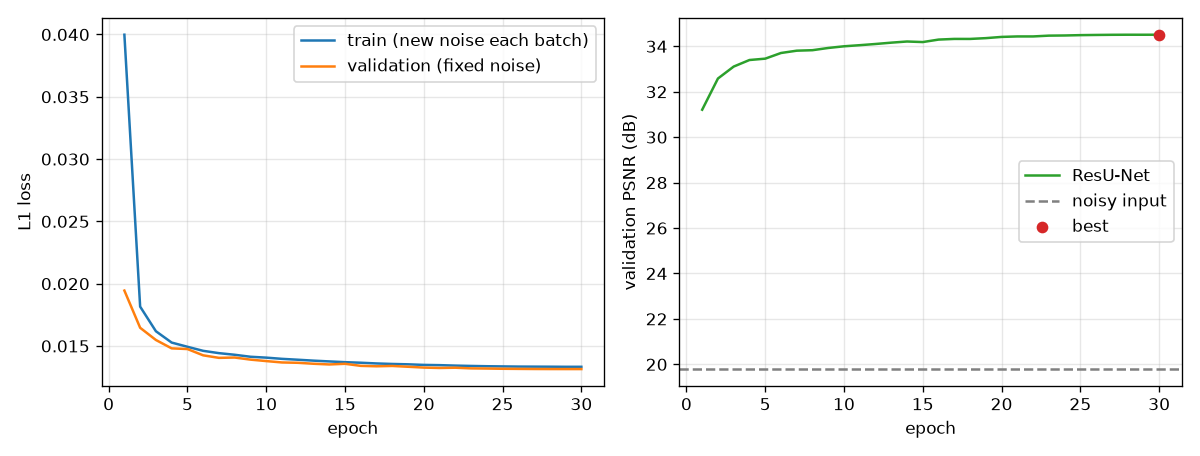
\includegraphics[width=0.9\linewidth]{figures/training_curves_medium.png}
\caption{ResU-Net training at the medium noise level. Left: $\ell_1$ loss on training batches (new noise every batch) and on the fixed noisy validation set. Right: validation PSNR per epoch; the dashed line is the PSNR of the noisy validation images and the dot marks the selected epoch.}
\label{fig:training}
\end{figure}

% ------------------------------------------------------------
\section{Preliminary Results}
\label{sec:results}
All results are on the \NTest{} test images at the medium noise level ($\lambda=50$, $\sigma=0.02$), with every method applied to the same fixed noisy images.

\begin{table}[htbp]
\centering
\caption{Main comparison (mean $\pm$ standard deviation over test images where applicable). Lost/New: pooled share of the classifier's clean findings that disappear / clean non-findings that become findings. Macro $\Delta$AUC: AUC drop against the labels, averaged over \NumAUCDiseases{} diseases, with paired-bootstrap 95\% CI; closer to 0 is better.}
\label{tab:main}
\resizebox{\linewidth}{!}{\begin{tabular}{@{}lccccccc@{}}
\toprule
\textbf{Method} & \textbf{PSNR (dB)} $\uparrow$ & \textbf{SSIM} $\uparrow$ & $\boldsymbol{\Delta p}$ $\downarrow$ & \textbf{Agr.} $\uparrow$ & \textbf{Lost} $\downarrow$ & \textbf{New} $\downarrow$ & \textbf{Macro $\Delta$AUC} \\
\midrule
Noisy (no denoising) & 19.77 $\pm$ 0.68 & 0.249 $\pm$ 0.069 & 0.2947 & 0.574 & 0.817 & 0.295 & $+0.158$ [$+0.096$, $+0.225$] \\
Median $3\times3$ & 26.77 $\pm$ 0.67 & 0.553 $\pm$ 0.070 & 0.3527 & 0.372 & 0.063 & 0.816 & $+0.143$ [$+0.090$, $+0.196$] \\
Anscombe-BM3D & 33.51 $\pm$ 0.99 & 0.884 $\pm$ 0.018 & 0.0961 & 0.805 & 0.107 & 0.224 & $+0.051$ [$+0.017$, $+0.080$] \\
ResU-Net (ours) & 34.47 $\pm$ 1.09 & 0.912 $\pm$ 0.017 & 0.0555 & 0.898 & 0.285 & 0.041 & $+0.017$ [$-0.005$, $+0.036$] \\
\bottomrule
\end{tabular}
}
\end{table}

\paragraph{Main findings.} Table~\ref{tab:main} and Fig.~\ref{fig:tradeoff} support four observations.
\begin{enumerate}[leftmargin=*]
  \item \textbf{Noise alone severely disrupts the classifier.} Without denoising, it loses \NoisyLost{} of its clean-image findings and its macro AUC drops by \NoisyDAUC{} \NoisyDAUCci.
  \item \textbf{Pixel fidelity and diagnostic preservation can disagree.} The median filter gains \MedianGain\,dB PSNR over the noisy input, yet its $\Delta p$ is \emph{worse} (\MedianDp{} vs.\ \NoisyDp) and it turns \MedianNew{} of the clean non-findings into findings. A PSNR-only evaluation would rank it as a clear improvement.
  \item \textbf{BM3D recovers most, but not all, diagnostic information.} Its $\Delta p$ falls to \BMDp, but its macro $\Delta$AUC of \BMDAUC{} \BMDAUCci{} excludes zero, so a measurable diagnostic loss remains.
  \item \textbf{ResU-Net is best on every averaged metric.} It reaches \OursPSNR\,dB and $\Delta p=\OursDp$, and its macro $\Delta$AUC of \OursDAUC{} \OursDAUCci{} is the only one whose interval includes zero.
\end{enumerate}

\begin{figure}[htbp]
\centering
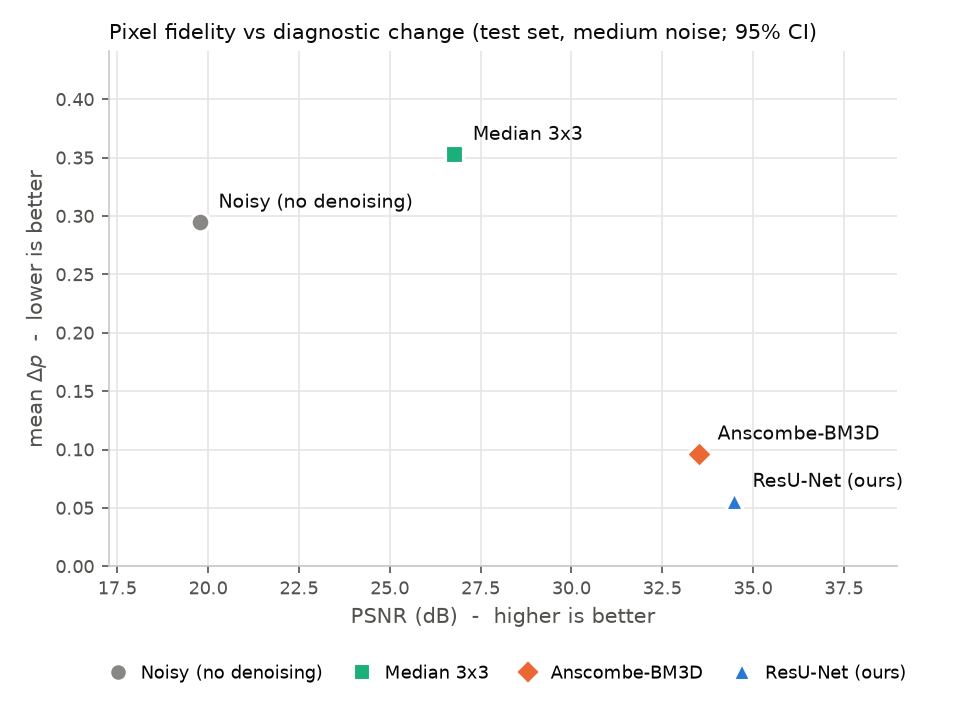
\includegraphics[width=0.68\linewidth]{figures/psnr_vs_delta_p_medium.png}
\caption{Pixel fidelity (PSNR, higher is better) against diagnostic change ($\Delta p$, lower is better) on the test set at medium noise, one point per method with 95\% confidence intervals (barely visible at this scale). The median filter moves right but also up: better pixels, worse diagnostic agreement.}
\label{fig:tradeoff}
\end{figure}

\paragraph{Paired comparison with BM3D.} Because both methods denoise the same images, we compare them per image (Table~\ref{tab:compare}). ResU-Net has a higher PSNR on \CmpPSNRShare{} of the images (\CmpPSNR\,dB \CmpPSNRci) and a lower $\Delta p$ on \CmpDpShare{} (\CmpDp{} \CmpDpci, a \CmpDpRel{} reduction). Its macro AUC is higher by \CmpAUC{} \CmpAUCci. The exception is lost findings, where BM3D is clearly better.

\begin{table}[htbp]
\centering
\caption{ResU-Net vs.\ Anscombe-BM3D on the same \NTest{} test images. Difference = ResU-Net minus BM3D, with paired-bootstrap 95\% CI; Wilcoxon signed-rank $p$ for per-image metrics; ``Better'' names the winner when the CI excludes 0. Arrows show which direction is better.}
\label{tab:compare}
\resizebox{\linewidth}{!}{\begin{tabular}{@{}lccccl@{}}
\toprule
\textbf{Metric} & \textbf{ResU-Net (ours)} & \textbf{Anscombe-BM3D} & \textbf{Difference [95\% CI]} & \textbf{Wilcoxon $p$} & \textbf{Better} \\
\midrule
PSNR (dB) $\uparrow$ & 34.47 & 33.51 & $+0.964$ [$+0.941$, $+0.988$] & $<0.001$ & ResU-Net \\
SSIM $\uparrow$ & 0.912 & 0.884 & $+0.027$ [$+0.027$, $+0.028$] & $<0.001$ & ResU-Net \\
$\Delta p$ $\downarrow$ & 0.0555 & 0.0961 & $-0.041$ [$-0.045$, $-0.036$] & $<0.001$ & ResU-Net \\
Agreement $\uparrow$ & 0.898 & 0.805 & $+0.093$ [$+0.080$, $+0.106$] & $<0.001$ & ResU-Net \\
Lost findings $\downarrow$ & 0.285 & 0.107 & $+0.178$ [$+0.156$, $+0.201$] & -- & Anscombe-BM3D \\
New findings $\downarrow$ & 0.041 & 0.224 & $-0.184$ [$-0.197$, $-0.170$] & -- & ResU-Net \\
Macro AUC $\uparrow$ & 0.724 & 0.690 & $+0.034$ [$+0.009$, $+0.057$] & -- & ResU-Net \\
\bottomrule
\end{tabular}
}
\end{table}

\paragraph{The two methods fail in opposite directions.} Averaged over all image-disease pairs, ResU-Net lowers the classifier's probabilities (mean change \OursShiftAll; \OursShiftFindings{} on the clean findings), while BM3D raises them (\BMShiftAll; \BMShiftNonFindings{} on the clean non-findings). Table~\ref{tab:findings} breaks this down by disease. ResU-Net makes the classifier miss findings, most strongly for nodules (\OursLostNodule{} lost vs.\ \BMLostNodule{} for BM3D). BM3D makes it report findings that were not there (for example \BMNewMass{} new mass findings vs.\ \OursNewMass{} for ResU-Net). Since nodules are small, low-contrast structures, this pattern is consistent with the $\ell_1$-trained network smoothing away fine texture, the risk anticipated in Milestone~1. The label-based nodule $\Delta$AUC of ResU-Net, \OursNoduleDAUC{} \OursNoduleDAUCci, shows no loss in \emph{ranking} quality. The classifier still orders patients correctly, but its nodule probabilities are shifted below the 0.5 operating point. In a deployed system with a fixed threshold, these would be missed findings, which averaged metrics such as $\Delta p$ and AUC do not reveal.

\begin{table}[htbp]
\centering
\caption{Lost and new findings per disease (share of the classifier's clean-image findings that disappear, and of its clean-image non-findings that become findings), sorted by the number of clean-image findings. Bold marks the lower (better) value of the two methods. Diseases with few clean findings (bottom rows) give unstable rates.}
\label{tab:findings}
\small
\begin{tabular}{@{}lrrrrr@{}}
\toprule
& \textbf{Clean} & \multicolumn{2}{c}{\textbf{Lost findings}} & \multicolumn{2}{c}{\textbf{New findings}} \\
\cmidrule(lr){3-4}\cmidrule(l){5-6}
\textbf{Disease} & \textbf{findings} & BM3D & ResU-Net & BM3D & ResU-Net \\
\midrule
Fibrosis & 369 & \textbf{2\%} & 19\% & 69\% & \textbf{11\%} \\
Infiltration & 268 & \textbf{13\%} & 25\% & 21\% & \textbf{5\%} \\
Mass & 267 & \textbf{0\%} & 8\% & 76\% & \textbf{25\%} \\
Nodule & 254 & \textbf{4\%} & 52\% & 52\% & \textbf{2\%} \\
Emphysema & 243 & \textbf{23\%} & 27\% & 26\% & \textbf{6\%} \\
Atelectasis & 141 & \textbf{8\%} & 35\% & 22\% & \textbf{3\%} \\
Pleural Thickening & 135 & \textbf{10\%} & 27\% & 38\% & \textbf{5\%} \\
Pneumothorax & 121 & \textbf{8\%} & 38\% & 27\% & \textbf{1\%} \\
Consolidation & 107 & \textbf{18\%} & 35\% & 13\% & \textbf{3\%} \\
Effusion & 85 & \textbf{11\%} & 26\% & 18\% & \textbf{3\%} \\
Cardiomegaly & 65 & 45\% & \textbf{37\%} & 2\% & \textbf{1\%} \\
Pneumonia & 20 & 50\% & 50\% & 0\% & \textbf{0\%} \\
Edema & 15 & \textbf{60\%} & 67\% & 0\% & 0\% \\
Hernia & 13 & 54\% & 54\% & 14\% & \textbf{3\%} \\
\bottomrule
\end{tabular}

\end{table}

\begin{table}[htbp]
\centering
\caption{Per-disease $\Delta$AUC (AUC on clean minus AUC after processing) with paired-bootstrap 95\% CI, for diseases with at least \MinPos{} test cases (number in brackets).}
\label{tab:dauc}
\resizebox{\linewidth}{!}{\begin{tabular}{@{}lcccc@{}}
\toprule
\textbf{Disease (cases)} & \textbf{Noisy (no denoising)} & \textbf{Median $3\times3$} & \textbf{Anscombe-BM3D} & \textbf{ResU-Net (ours)} \\
\midrule
Atelectasis (47) & $+0.192$ [$+0.084$, $+0.295$] & $+0.215$ [$+0.113$, $+0.328$] & $+0.026$ [$-0.016$, $+0.065$] & $+0.019$ [$-0.011$, $+0.049$] \\
Effusion (38) & $+0.269$ [$+0.182$, $+0.360$] & $+0.150$ [$+0.074$, $+0.237$] & $+0.065$ [$+0.029$, $+0.105$] & $+0.050$ [$+0.019$, $+0.084$] \\
Infiltration (50) & $+0.059$ [$-0.021$, $+0.143$] & $+0.149$ [$+0.060$, $+0.237$] & $+0.035$ [$-0.010$, $+0.084$] & $+0.009$ [$-0.025$, $+0.046$] \\
Nodule (21) & $+0.068$ [$-0.107$, $+0.237$] & $+0.146$ [$-0.036$, $+0.320$] & $+0.036$ [$-0.061$, $+0.125$] & $-0.020$ [$-0.086$, $+0.038$] \\
Pleural Thickening (20) & $+0.204$ [$+0.037$, $+0.386$] & $+0.056$ [$-0.033$, $+0.155$] & $+0.090$ [$+0.003$, $+0.168$] & $+0.025$ [$-0.026$, $+0.071$] \\
\midrule
\textit{Macro average} & $+0.158$ [$+0.096$, $+0.225$] & $+0.143$ [$+0.090$, $+0.196$] & $+0.051$ [$+0.017$, $+0.080$] & $+0.017$ [$-0.005$, $+0.036$] \\
\bottomrule
\end{tabular}
}
\end{table}

\paragraph{Qualitative examples.} Examples are chosen by fixed rules rather than by hand: the image with the median ResU-Net PSNR, the median-PSNR image among those labelled Nodule or Mass, and the image with the largest ResU-Net $\Delta p$. The zoom box is placed where the clean image has the most local detail. Figures~\ref{fig:qual2} and~\ref{fig:qual3} show the last two; the typical example is in the repository.

\begin{figure}[htbp]
\centering
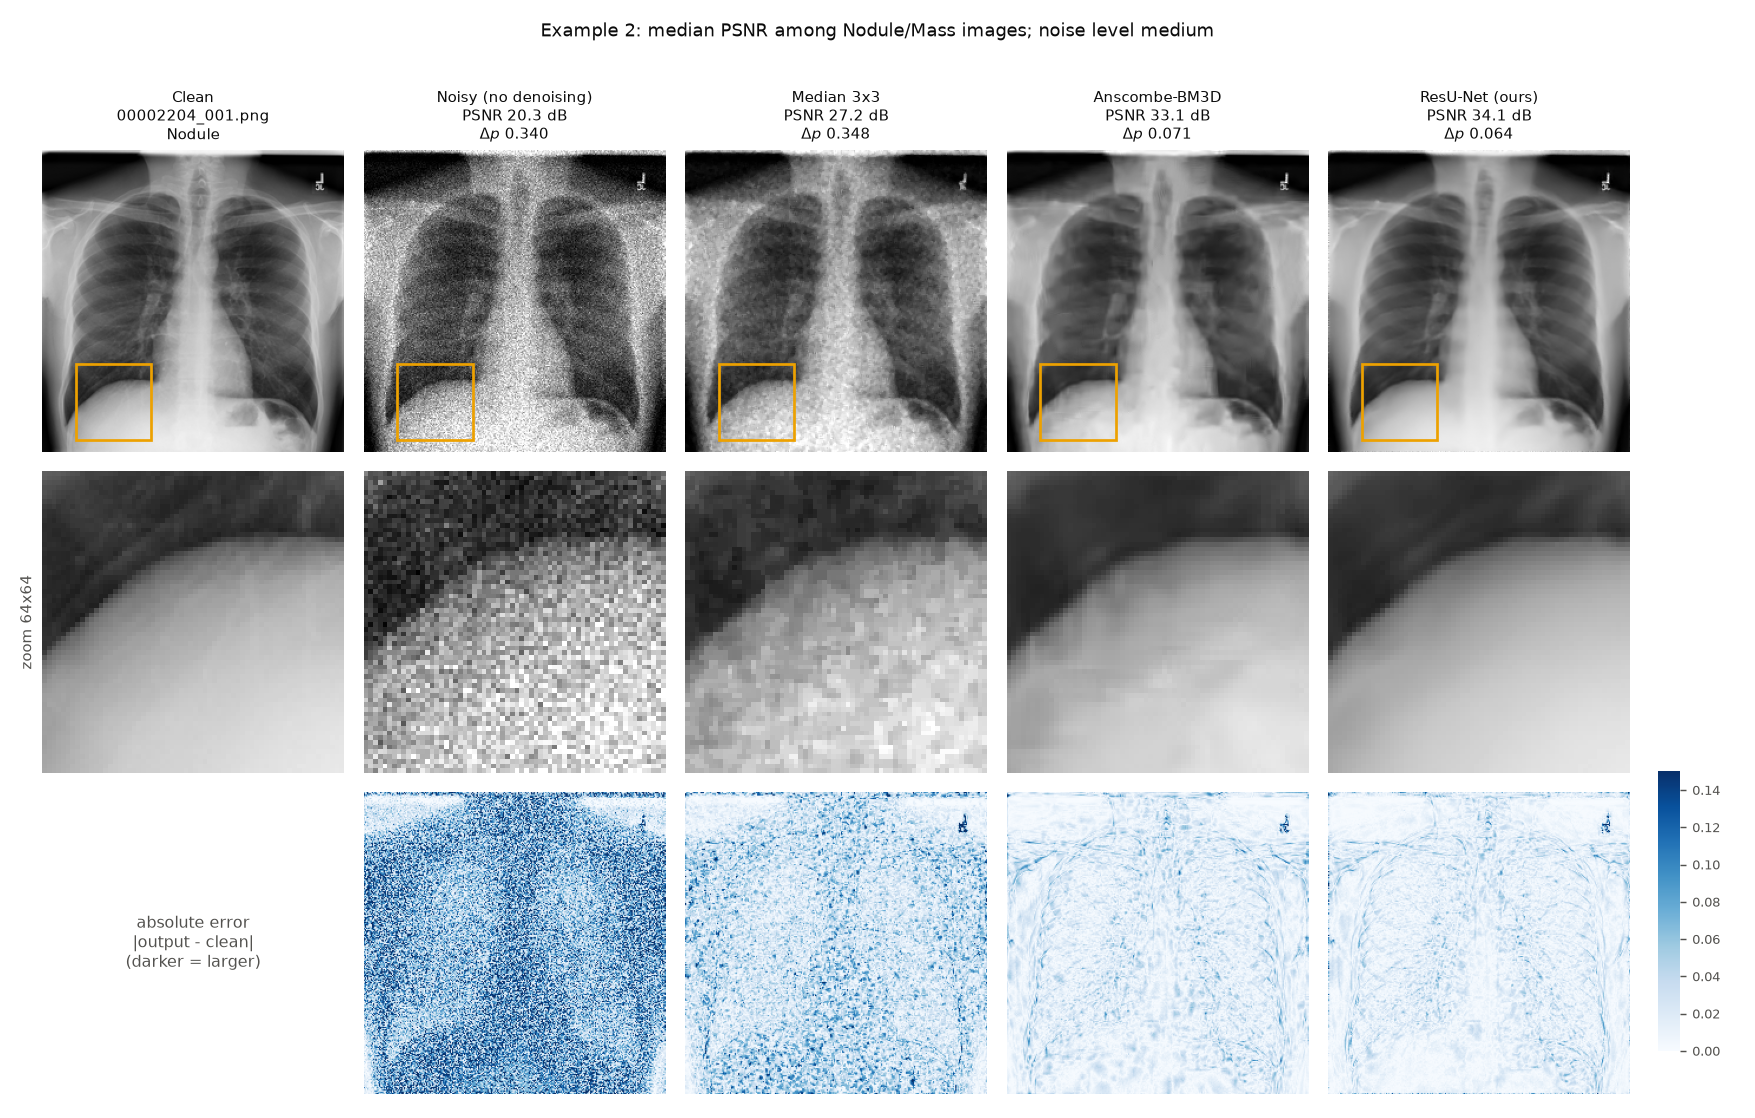
\includegraphics[width=\linewidth]{figures/qualitative_medium_2_small_finding.png}
\caption{Image labelled Nodule (median PSNR among Nodule/Mass test images). Rows: full image with the zoom region marked, $64\times64$ zoom, absolute error $|\hat{x}-x|$. Both BM3D and ResU-Net remove the noise; in the zoom, BM3D leaves blotchy structured texture while ResU-Net is smoother. Per-image PSNR and $\Delta p$ are in the panel titles.}
\label{fig:qual2}
\end{figure}

\begin{figure}[htbp]
\centering
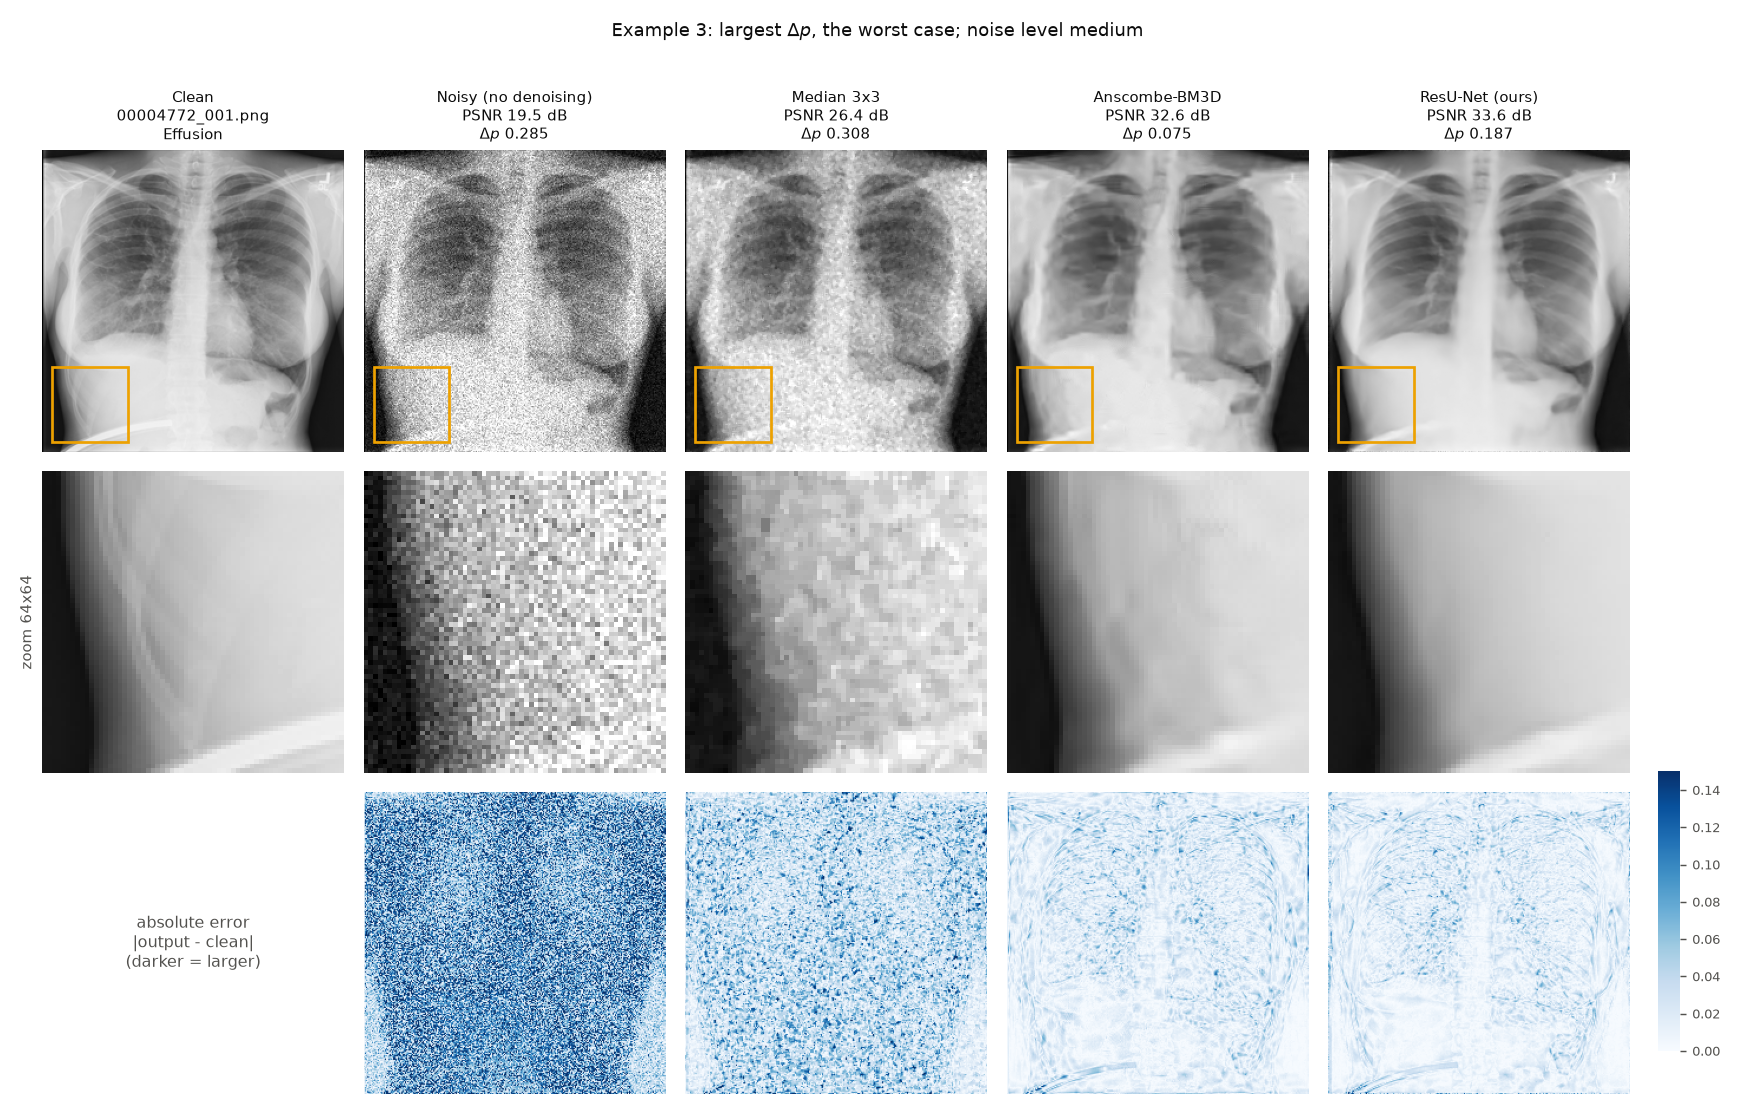
\includegraphics[width=\linewidth]{figures/qualitative_medium_3_worst_case.png}
\caption{Worst case for ResU-Net (largest $\Delta p$ on the test set; image labelled Effusion). In the zoom, the faint oblique edges visible in the clean image are largely removed by ResU-Net and partly kept by BM3D; on this image BM3D changes the classifier less (panel titles). This is an example of the oversmoothing behind ResU-Net's lost findings.}
\label{fig:qual3}
\end{figure}

\paragraph{Effect of the noise level on the classifier.} Table~\ref{tab:judgelevels} shows the classifier on the noisy test images (no denoising) at the three levels. Lost findings (\JudgeLowLost, \JudgeMediumLost, \JudgeHighLost) and macro $\Delta$AUC (\JudgeLowDAUC, \JudgeMediumDAUC, \JudgeHighDAUC) grow with the noise level. $\Delta p$ does not (\JudgeLowDp, \JudgeMediumDp, \JudgeHighDp): already at our lowest level the classifier's outputs have moved about as far as they go, so $\Delta p$ is not a usable severity measure for these noise levels. We therefore use lost findings and $\Delta$AUC to describe noise severity.

\begin{table}[htbp]
\centering
\caption{The frozen classifier on noisy test images without denoising, per noise level.}
\label{tab:judgelevels}
\begin{tabular}{@{}lccccc@{}}
\toprule
\textbf{Noise level} & $\boldsymbol{\Delta p}$ & \textbf{Agr.} & \textbf{Lost} & \textbf{New} & \textbf{Macro $\Delta$AUC [95\% CI]} \\
\midrule
Low & 0.294 & 0.551 & 73.5\% & 35.3\% & $+0.114$ [$+0.059$, $+0.173$] \\
Medium & 0.295 & 0.574 & 81.7\% & 29.5\% & $+0.158$ [$+0.098$, $+0.224$] \\
High & 0.280 & 0.602 & 86.4\% & 24.2\% & $+0.194$ [$+0.130$, $+0.260$] \\
\bottomrule
\end{tabular}

\end{table}

% ------------------------------------------------------------
\section{Challenges \& Deviations from the M1 Plan}
\label{sec:challenges}
\begin{itemize}[leftmargin=*]
  \item \textbf{Errors in the noise and Anscombe code (fixed).} The M1 implementation applied the Anscombe transform to $[0,1]$ intensities instead of photon counts, so the noise was not stabilized (after the transform its standard deviation was far below 1 and changed with brightness). The formula in the M1 report had the same error. The algebraic inverse used in M1 is biased: our noise report measured a darkening of about 0.005 at the medium level, against less than 0.001 for the unbiased inverse. The noisy image was clipped to $[0,1]$ before the transform, and a single fixed seed gave every image the same noise pattern. All four issues were fixed (Section~\ref{sec:data}--\ref{sec:baselines}) and are now covered by tests. The M1 bibliography entry for \citet{makitalo2013gat} was also corrected (it combined the 2013 paper's title with the 2011 paper's details).
  \item \textbf{Noise levels.} M1 estimated noisy-image PSNRs of about 30/24/19\,dB. The measured values on our test images are \NoiseLowPSNR/\NoiseMediumPSNR/\NoiseHighPSNR\,dB (Table~\ref{tab:noise}). The $(\lambda,\sigma)$ values were taken from the M1 plan and not calibrated to clinical contrast-to-noise ratios as M1 suggested; they are strong noise levels, and conclusions are limited to this simulation.
  \item \textbf{Subset selection.} Images come from the first three archive folders rather than the whole dataset, and patients were selected in a seeded random order with at most \MaxPerPatient{} images each (M1 described hashing patient IDs). This yields \NPatients{} patients (M1 estimated about 1{,}880) and a healthier-than-average subset (Section~\ref{sec:data}). Patient IDs are not linked to diagnoses, so we do not expect this choice to bias the comparison between methods, but the absolute numbers are specific to this subset.
  \item \textbf{Few positive cases.} Label-based $\Delta$AUC is limited to \NumAUCDiseases{} diseases with at least \MinPos{} test cases (we lowered our initial threshold of 25, which left only three), and is always reported with confidence intervals.
  \item \textbf{Extended metrics.} Because $\Delta p$ does not grow with noise at our levels (Table~\ref{tab:judgelevels}) and does not show the direction of changes, we added lost/new findings and paired statistical comparisons. Without them, ResU-Net's loss of nodule findings would not have been visible.
  \item \textbf{Smaller deviations.} The network has \Params{} parameters (M1 estimated about 384{,}000 for the same design). Training was much faster than planned (\TrainMinutes\,minutes instead of about 36), while BM3D was slower (\BMSec\,s per image with parallel workers, against an estimated 1.5\,s).
  \item \textbf{Team.} \todo{Describe how the M2 work}
\end{itemize}

% ------------------------------------------------------------
\section{Updated Work Breakdown \& MVP Status}
\label{sec:workbreakdown}
\paragraph{MVP status: reached.} All four MVP items from Milestone~1 are complete: (1) the Poisson-Gaussian noise pipeline with fixed evaluation sets; (2) verified Anscombe-BM3D and median baselines; (3) a fully trained ResU-Net at medium noise; and (4) the comparison on the \NTest{} test images with PSNR, SSIM, $\Delta p$ and agreement (Table~\ref{tab:main}). Beyond the MVP, we added $\Delta$AUC with confidence intervals, lost/new findings, paired statistical tests, and the per-disease analysis that M1 listed as a stretch goal (Table~\ref{tab:findings}).

\begin{table}[htbp]
\centering
\caption{Updated milestone task allocation.}
\label{tab:tasks}
\begin{tabular}{@{}p{0.16\linewidth}p{0.39\linewidth}p{0.39\linewidth}@{}}
\toprule
\textbf{Milestone} & \textbf{Omar Hesham Nasr (2401812)} & \textbf{Mohamed Ahmed Abdelsalaam (2400033)} \\
\midrule
M2 (Wk 6) \newline completed & \todo{what was done} & \todo{what was done} \\
\midrule
M3 (Wk 9) \newline planned & \todo{task} & \todo{task} \\
\bottomrule
\end{tabular}
\end{table}

% ------------------------------------------------------------
\section{Next Steps}
\label{sec:next}
\begin{itemize}[leftmargin=*]
  \item \textbf{Week 7: noise-level ablation.} Train and evaluate ResU-Net and BM3D at the low and high levels. Optionally add a milder level to locate where the classifier starts to lose findings, since even our lowest level disrupts it strongly.
  \item \textbf{Week 7--8: diagnostic loss (stretch goal from M1).} Train with $\mathcal{L}=\|\hat{x}-x\|_1+\gamma\,\|g(\hat{x})-g(x)\|_1$ using the frozen classifier's features, and test whether it reduces lost findings (especially nodules) without giving up PSNR. This is the ablation isolating our main design choice.
  \item \textbf{Week 8: robustness of the result.} Repeat training with three seeds, and check whether the lost findings are a threshold effect, by comparing operating points per disease.
  \item \textbf{Week 9:} final report (template 6.3), README, demo, and presentation.
\end{itemize}

\paragraph{AI-tool usage.} Code scaffolding, tests and a first draft of this report's text were written with AI assistance (Claude, Anthropic). All experiments were run by the team on our own hardware, every number in this report is produced by the repository's scripts from those runs, and the text was reviewed and edited by the team.

\bibliographystyle{unsrtnat}
\bibliography{references}

\end{document}
